\lecture{2009-10-21}

\subsection{Ungleichungen,  Betrag Kalkül-Teil}
Definition: Unter einer Ungleichung für reelle Zahlen $x,y$ verstehen wir einen Größenvergleich
\begin{center}
% use packages: array
\begin{tabular}{lll}
$x<y$ & ``kleiner $<$'' & kleiner $\leq$ \\ 
$x>y$ & ``größer $>$'' & größer $\geq$
\end{tabular}
\end{center}

Abschätzung: $x<y$ heißt Größe von $x$ durch Größe von $y$ abschätzen. Regelwerk für Abschätzungen (Anordnungsaxiome)
$\leadsto$ Zahlengerade.
\begin{enumerate}
 \item $x \leq y, a\leq b \Rightarrow x+a \leq y+b$
 \item $x<y, 0 \leq a \Rightarrow ax \leq ay$
 
$x<y, 0 < a \Rightarrow ax < ay$
 \item $0<x\leq y \Rightarrow 0 < \frac{1}{y} \leq \frac{1}{x}$
\end{enumerate}
Typische Aufgabe:
lege $a$ fest mit Eigenschaft
\begin{align*}
-3a-2 &\leq 5 &\leq -3a+4 \\
-3a\leq 7 & & 1 \leq -3a \\
-\frac{1}{3} &\leq a &\leq -\frac{7}{3}
\end{align*}

Definition: $S \subset \mathbb{R}$ heißt nach oben beschränkt, falls eine Zahl $b$ existiert mit $S\subseteq ]-\infty,b]$ ``$b$ obere Schranke von $S$''

Definition: Ist $S \subseteq \mathbb{R}$ nach oben beschränkt, so heißt die kleinste obere Schranke von $S$ das \emph{Supremum} $s:=\sup S$

analog: \emph{Infimum}: ``größte unter Schranke'' $u := \inf S$

Bemerkung: kleinste obere Schranke muss nicht element von $S$ sein, das \emph{Maximum} schon

\begin{itemize}
 \item $\sup \{x \in \mathbb{Q} | x^2 < 2 \} = \sqrt{2} \notin \mathbb{Q}$
 \item $\sup \{[a,b]\} = b \in [a,b]$
 \item $\inf \{ 1+\frac{1}{n}|n\in \mathbb{N}\} = 1$
\end{itemize}

Vollständigkeitsaxiom für $\mathbb{R}$
Jede nach oben beschränkte Menge reeller Zahlen besitzt ein \emph{Supremum}.$\mathbb{R}$ überabzählbar, $\mathbb{Q}$ abzählbar (siehe Bornemann)

Definition: Betrag $|a|, a \in \mathbb{R}$
$|a|=a \textrm{falls} a \geq 0 \land -a \textrm{falls} a<0$

Rechenregeln(Beträge):
\begin{itemize}
 \item $-|a|\leq a \leq |a|$
 \item $-|a| = |a|$
 \item $|ab| = |a||b|$
 \item $|\frac{a}{b}| = \frac{|a|}{|b|}, b\neq 0$
\end{itemize}

Anwendung: Dreiecksungleichung
z.z.: $|a+b| \leq |a|+|b|$. Dazu
\begin{align*}
-|a|&\leq a &\leq |a| \\
-|b|&\leq b &\leq |b| \\
\Rightarrow -(|a|+|b|)&\leq a+b &\leq |a|+|b| \\
-(|a|+|b|)&\leq |a+b| &\leq |a|+|b|
\end{align*}
Abstandsmessung $|x-a| \leq \epsilon$

Rechenbeispiel:
% Rechenbeispiel in der vorh. Version war offensichtlich falsch. Ich hab die Aufgabenstellung so
% angepasst, dass die Lösungsmenge nun korrekt sein sollte.
%$x\in \mathbb{R}$ gesucht mit $\frac{3}{x-9} \leq \frac{2}{x+2}$. Nenner $x\neq9 \land x\neq -2$
$x\in \mathbb{R}$ gesucht mit $\frac{3}{|x-9|} > \frac{2}{x+2}$. Nenner $x\neq9 \land x\neq -2$

(Zahlenstrahl mit Markierung von -2 nach links und Markierung von 9 nach rechts)

\begin{align*}
M_1 &= \{x \in \mathbb{R} | x < -2\} \\
M_2 &= \{x \in \mathbb{R} | -2 < x < 9\} \\
M_3 &= \{x \in \mathbb{R} | x > 9\}
\end{align*}

\begin{itemize}
 \item Diskussion von $M_1: x < -2$
\begin{align*}
|x-9|>0 &\Rightarrow \frac{3}{|x-9|} > 0 \\
x<-2 &\Rightarrow x+2<0 \Rightarrow \frac{2}{x+2}<0
\end{align*}
ganz $M_1$ zulässig
 \item Diskussion von $M_2: -2<x<9$
\begin{align*}
\Rightarrow &x+2 > 0 \\
&x-9<0 \textrm{d.h.} |x-9|=9-x \\
\textrm{zu prüfen:}
\frac{3}{9-x} > \frac{2}{x+2} \textrm{Betrag weg} \\
3x+6 > 18-2x \\
x > \frac{12}{5} = 2 \frac{2}{5}
\textrm{erlaubt:} \frac{12}{5}<x<9
\end{align*}
 \item Diskussion von $M_3: x>9$
\begin{align*}
 \Rightarrow \underbrace{|x-9|}_{>0} = x-9 \\
\frac{3}{x-9} > \frac{2}{x+2}
\Rightarrow x>-24
\end{align*}
$M_3$ zulässig

Ergebnis: $\{x|x<-2, \frac{12}{5}<x<9, 9<x\}$
\end{itemize}

\begin{minipage}{1\textwidth}
Anwendung: Geometrie
\begin{align*}
M = \{(x,y)| |x|+|y| \leq 1 \} x,y \in \mathbb{R} \\
|x|+|y| \leq 1 \Rightarrow &x \geq 0, y \geq 0: x+y \leq 1 \Rightarrow y \leq 1-x \\
	&x \geq 0, y < 0: x-y \leq 1 \Rightarrow y \geq -1+x \\
	&x < 0, y \geq 0: -x+y \leq 1 \Rightarrow y \leq 1+x \\
	&x < 0, y < 0: -x-y \leq 1 \Rightarrow y \geq -1-x \\
\end{align*}

\begin{center}
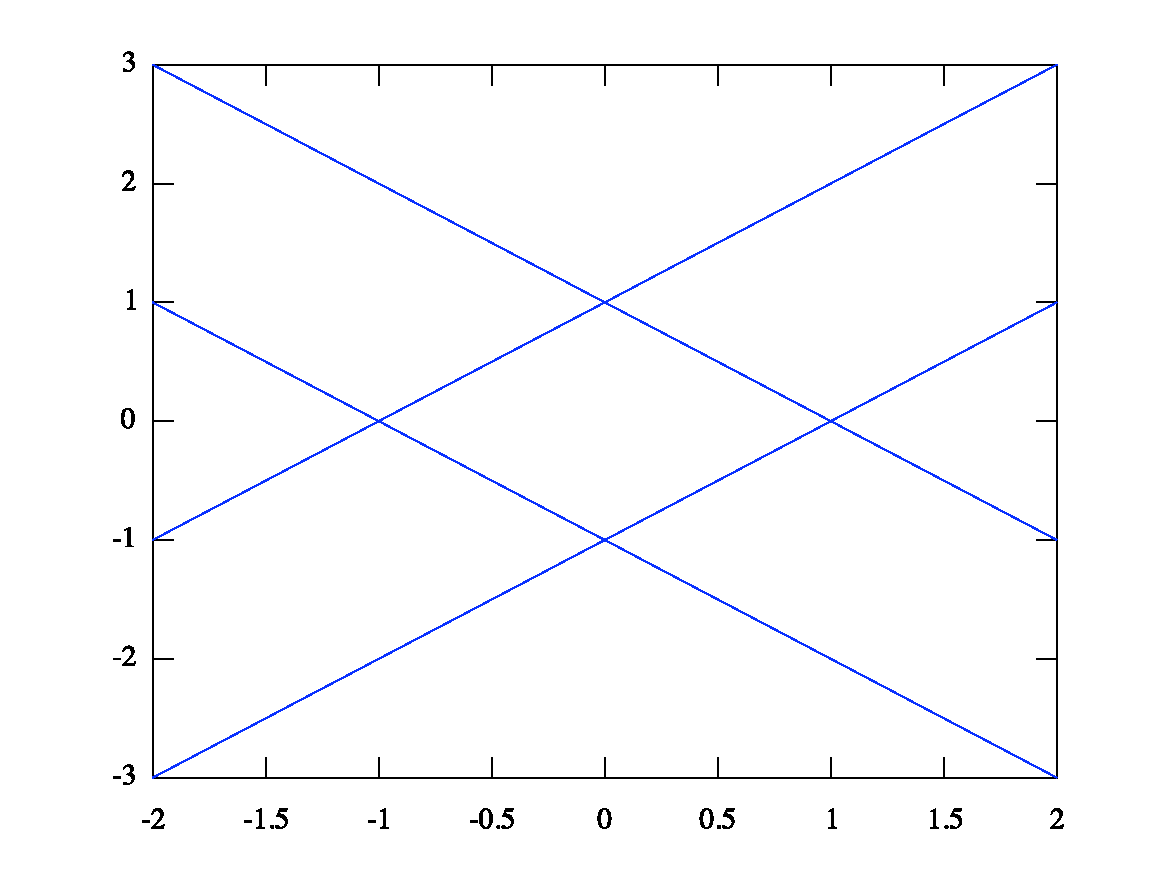
\includegraphics[width=0.6\textwidth]{geo_betraege.pdf}
\captionof{figure}{Geometrische interpretation von $|x|+|y| \leq 1$}
\end{center}
\end{minipage}
  
\medskip Kreis um Ursprung mit Fläche
Radius $\{(x,y)| x^2+y^2\leq r^2 \}$

Kreislinie $\{(x,y)| x^2+y^2 = r^2 \}$

